\documentclass[11pt]{article}

\usepackage{geometry}
 \geometry{
 letterpaper,
 left=1in,
 right=1in,
 bottom=1in,
 top=1.25in
 }               % See geometry.pdf to learn the layout options. There are lots.
%\geometry{landscape}                
\usepackage{graphicx}
\usepackage{amssymb}
\usepackage{epstopdf}
\DeclareGraphicsRule{.tif}{png}{.png}{`convert #1 `dirname #1`/`basename #1 .tif`.png}
\usepackage{url}
\usepackage{amsmath}
\usepackage{mathtools}
\usepackage{booktabs}
\usepackage[format=hang,labelfont=bf]{caption}
\usepackage{float}
\usepackage[parfill]{parskip}
\usepackage{tensor}
\usepackage{natbib}
\usepackage[inline]{enumitem}
%\begin{enumerate*}%[label=\textit{\alph*)}] 
%\item
%\end{enumerate*} 
\usepackage{color}

% Appendices - nice table/figure numbering with appendix identifier
\usepackage[titletoc,toc,title]{appendix}
%% Restart table/figure numbering in appendices using <\counterwithin{figure}{section}>
%\usepackage{chngcntr}

\usepackage[parfill]{parskip}

\usepackage{url}
%\usepackage{hyperref}
\usepackage{authblk}
\renewcommand\Affilfont{\footnotesize}
\usepackage{easymat}
\usepackage{bigstrut}
\usepackage{threeparttable} 
\usepackage[format=hang,labelfont=bf]{caption}
\usepackage{rotating}
\usepackage{subfig}
\usepackage{wrapfig}
\usepackage{mdframed}
\usepackage[raggedright]{titlesec}
\usepackage{longtable}

\usepackage{array}
\newcolumntype{L}[1]{>{\raggedright\let\newline\\\arraybackslash\hspace{0pt}}m{#1}}
\newcolumntype{C}[1]{>{\centering\let\newline\\\arraybackslash\hspace{0pt}}m{#1}}
\newcolumntype{R}[1]{>{\raggedleft\let\newline\\\arraybackslash\hspace{0pt}}m{#1}}

\usepackage{scrextend}
\deffootnote[1em]{1em}{1em}{\textsuperscript{\thefootnotemark}}

\usepackage[table, dvipsnames]{xcolor}
\definecolor{lightgray}{gray}{0.95}
\definecolor{white}{rgb}{1.0, 1.0, 1.0}

% for making changes in response to reviews
% must come *after* xcolor
% toggle the following two lines to reveal or hide the changes
%\usepackage[commentmarkup=footnote]{changes}
\usepackage[final]{changes}
\definechangesauthor[name={Reviewer 1}, color=blue]{r1}
\definechangesauthor[name={Reviewer 2}, color=blue]{r2}
\definechangesauthor[name={Reviewer 3}, color=blue]{r3}
\definechangesauthor[name={Reviewer 4}, color=OliveGreen]{r4}
\definechangesauthor[name={Reviewer 5}, color=OliveGreen]{r5}
\definechangesauthor[name={Editors}, color=Violet]{editors}
\definechangesauthor[name={Notes}, color=brown]{note}

\DeclareMathOperator{\Tr}{Tr}

\newcommand{\mbf}{\mathbf}

\newcommand{\qf}{\tensor*[_5]{\mbox{q}}{_0}}
\newcommand{\qoz}{\tensor*[_1]{\mbox{q}}{_0}}
\newcommand{\qoo}{\tensor*[_1]{\mbox{q}}{_1}}
\newcommand{\qfo}{\tensor*[_4]{\mbox{q}}{_1}}
\newcommand{\qof}{\tensor*[_1]{\mbox{q}}{_4}}
\newcommand{\qff}{\tensor*[_{45}]{\mbox{q}}{_{15}}}
\newcommand{\qox}{\tensor*[_{1}]{\mbox{q}}{_{x}}}
\newcommand{\qoa}{\tensor*[_{1}]{\mbox{q}}{_{a}}}
\newcommand{\qfx}{\tensor*[_{5}]{\mbox{q}}{_{x}}}
\newcommand{\qnx}{\tensor*[_{n}]{\mbox{q}}{_{x}}}
\newcommand{\qts}{\tensor*[_{20}]{\mbox{q}}{_{60}}}
\newcommand{\qfxhat}{\tensor*[_{5}]{\widehat{\mbox{q}}}{_{x}}}

\newcommand{\ez}{{\mbox{e}}{_0}}
\newcommand{\ezhat}{{\widehat{\mbox{e}}}{_0}}
\newcommand{\ex}{{\mbox{e}}{_x}}
\newcommand{\exhat}{{\widehat{\mbox{e}}}{_x}}

\newcommand{\mfx}{\tensor*[_{5}]{\mbox{m}}{_{x}}}
\newcommand{\mfz}{\tensor*[_{5}]{\mbox{m}}{_{0}}}

\newcommand{\anx}{\tensor*[_{n}]{\mbox{a}}{_{x}}}
\newcommand{\aoz}{\tensor*[_{1}]{\mbox{a}}{_{0}}}
\newcommand{\alast}{\tensor*[_{+}]{\mbox{a}}{_{110}}}

\newcommand{\lx}{\tensor*[_{}]{\mbox{l}}{_{x}}}

\newcommand{\logit}{\mbox{logit}}
\newcommand{\expit}{\mbox{expit}}

% Insert labels and numbers into complex align environment equations, e.g. matrices of equations
\makeatletter
\newcommand\Label[1]{&\refstepcounter{equation}(\theequation)\ltx@label{#1}&}
\makeatother

%double space
\usepackage{setspace}
%\linespread{1.5}

%touch-up footnote formatting
\usepackage{scrextend}
\deffootnote[1em]{1em}{1em}{\textsuperscript{\thefootnotemark}}

%% Fonts
% sans-serif
\renewcommand{\familydefault}{\sfdefault}
% Helvetica
\usepackage{helvet}
% mathmode fonts sans-serif too
\usepackage[italic]{mathastext}
% 'isomath' sets upper case greek letters italic in accordance with 
% the International Standard ISO 80000-2
\usepackage{isomath}

\sloppy

% remove extra spaces after using \input{}
\newcommand{\lineinput}[1]{%
  \begingroup\endlinechar=-1 \input{#1}\endgroup
}

% reference the appendices in separate file
\usepackage{xr}
\externaldocument{"SVD-Comp-Manuscript"}



\title{\vfill Appendix \\[10pt] A General Age-Specific Mortality Model with An Example Indexed by Child or Both Child and Adult Mortality}

\author[1,2,*]{Samuel J. Clark}

\affil[1]{Department of Sociology, The Ohio State University}
\affil[2]{MRC/Wits Rural Public Health and Health Transitions Research Unit (Agincourt), School of Public Health, Faculty of Health Sciences, University of the Witwatersrand}
\affil[*] {Contact: work@samclark.net, 206.303.9620}

%\date{\today \vfill}
\date{2022 \vfill}

\begin{document}

\pagenumbering{roman} 
\maketitle

\linespread{1}

\newpage
\pagenumbering{arabic} 
\renewcommand*{\thepage}{A\arabic{page}}

%%% === %%% === %%%
\begin{appendices}
\counterwithin{figure}{section} % restarts figure label and inserts appendix counter in label
\counterwithin{table}{section}
\counterwithin{equation}{section}


%%% === %%% === %%%
\section{SVD Algebra} \label{app:svd}

Below I rearrange the basic SVD relationship to derive useful additional relationships.  $\mbf{X}$ is an $A  \times L$ matrix of rank $\rho$.%
\begin{align}
\mbf{X}
&=% 1 
\mbf{USV}^\text{T} 
\\
\left[ 
	\begin{matrix}
	| & & | \\
	\mbf{x}_{1} & \ldots  & \mbf{x}_{L}  \\
	| & & | \\
	\end{matrix}
\right] 
&=% 2
\left[ 
	\begin{matrix}
	| & & | \\
	\mbf{u}_{1} & \ldots  & \mbf{u}_{\rho}  \\
	| & & |  \\
	\end{matrix}
\right]  
\left[ 
	\begin{matrix}
		s_{1} & \ldots & 0  \\
		\vdots & \ddots & \vdots \\
		0 & \ldots & s_{\rho}  \\
	\end{matrix}
\right]
\left[ 
	\begin{matrix}
		\text{---} & \mbf{v}_1 & \text{---} \\
		& \vdots  & \\
		\text{---} & \mbf{v}_\rho & \text{---} \\
	\end{matrix}
\right] 	 
\nonumber \\
&=% 3
\left[ 
	\begin{matrix}
		| & & | \\
	\mbf{u}_{1} & \ldots  & \mbf{u}_{\rho}  \\
		| & & | \\
	\end{matrix}
\right]  
\left[ 
	\begin{matrix}
		\text{---} & s_{1} \mbf{v}_1 & \text{---} \\
		& \vdots & \\
		\text{---} & s_{\rho} \mbf{v}_\rho & \text{---} \\
	\end{matrix}
\right] 	 
\nonumber \\
&=% 4
\left[ 
	\begin{matrix}
		\sum_{i=1}^{\rho} u_{1i} s_{i} v_{1i} & \ldots & \sum_{i=1}^{\rho} u_{1i} s_{i} v_{Li} \\
		\vdots & \ddots  & \vdots \\		
		\sum_{i=1}^{\rho} u_{Ai} s_{i} v_{1i} & \ldots & \sum_{i=1}^{\rho} u_{Ai} s_{i} v_{Li} \\
	\end{matrix}
\right]  
\nonumber \\
&=% 5
\left[ 
	\begin{matrix}
		| & & | \\
		\sum_{i=1}^{\rho} s_{i} v_{1i} \mbf{u}_{i}  & \ldots & \sum_{i=1}^{\rho} s_{i} v_{Li} \mbf{u}_{i}  \\
		| & & | \\
	\end{matrix}
\right] 
\label{eq:appB:genComponents} \\ 
&=% 6
\sum_{i=1}^{\rho} \left[ 
	\begin{matrix}
		| & & | \\
		s_{i} v_{1i} \mbf{u}_{i}  & \ldots  & s_{i} v_{Li} \mbf{u}_{i} \\
		| & & | \\
	\end{matrix}
\right] 
\nonumber \\
&=% 7
\sum_{i=1}^{\rho} \left[ 
	\begin{matrix}
		s_{i} v_{1i} u_{1i} & \ldots & s_{i} v_{Li} u_{1i} \\
		\vdots & \ddots & \vdots \\
		s_{i} v_{1i} u_{Ai}  & \ldots  & s_{i} v_{Li} u_{Ai} \\
	\end{matrix}
\right] 
\nonumber \\
&=% 8
\sum_{i=1}^{\rho}
s_{i} 
\left[ 
	\begin{matrix}
		u_{1i} \\
		\vdots \\
		u_{Ai} \\
	\end{matrix}
\right]  
\left[ 
	\begin{matrix}
		v_{1i} \ldots v_{Li} \\
	\end{matrix}
\right] 
\label{eq:appB:XsumRank-1Detail} \\
\mathbf{X} &=% 9
\sum_{i=1}^{\rho} s_{i} \mbf{u}_{i} \mbf{v}_{i}^\text{T}
\label{eq:appB:XsumRank-1}
\end{align}%

From Equation \ref{eq:appB:genComponents} we have
\begin{align}
\mbf{x}_{\ell} = \sum_{i=1}^{\rho} s_{i} v_{\ell i} \mbf{u}_{i} \ .
\label{eq:appB:cols}
\end{align}%


%%% === %%% === %%%
\newpage
\section{SVD Component Values} \label{app:comps}

\begingroup
\renewcommand\arraystretch{1.0}
\rowcolors{1}{}{lightgray}
\begin{centering}
\def\sym#1{\ifmmode^{#1}\else\(^{#1}\)\fi}
\begin{longtable}{rrrrrrrrr} 
\hiderowcolors
\caption{SVD Component ($s_{z i} \mathbf{u}_{z i}$) Values.} \label{tab:appA:comps} \\
\showrowcolors
  \toprule
\hiderowcolors
 & \multicolumn{4}{c}{Female} &  \multicolumn{4}{c}{Male} \\
  \cmidrule(lr){2-5} \cmidrule(lr){6-9}
 Age & \multicolumn{1}{c}{$c_1$} & \multicolumn{1}{c}{$c_2$} & \multicolumn{1}{c}{$c_3$} & \multicolumn{1}{c}{$c_4$} & \multicolumn{1}{c}{$c_1$} & \multicolumn{1}{c}{$c_2$} & \multicolumn{1}{c}{$c_3$} & \multicolumn{1}{c}{$c_4$} \\
\showrowcolors 
  \midrule
\endfirsthead

\hiderowcolors
\multicolumn{9}{c}%
{{\bfseries \tablename\ \thetable{} -- continued from previous page}} \\
  \toprule
 & \multicolumn{4}{c}{Female} &  \multicolumn{4}{c}{Male} \\
  \cmidrule(lr){2-5} \cmidrule(lr){6-9}
 Age & \multicolumn{1}{c}{$c_1$} & \multicolumn{1}{c}{$c_2$} & \multicolumn{1}{c}{$c_3$} & \multicolumn{1}{c}{$c_4$} & \multicolumn{1}{c}{$c_1$} & \multicolumn{1}{c}{$c_2$} & \multicolumn{1}{c}{$c_3$} & \multicolumn{1}{c}{$c_4$} \\ 
\showrowcolors
  \midrule
\endhead

\bottomrule 
\rowcolor{white} \multicolumn{9}{c}{{continued on next page}} 
\endfoot

\bottomrule
\endlastfoot

\input ../tables/us.txt

\end{longtable}
\end{centering}
\endgroup


%%% === %%% === %%%
\newpage
\section{SVD Sum of Squares and SVD-Comp Calibration using HMD Data} \label{app:variances}

\added[id=r1]{The \textit{total sum of squares} explained by each component of the SVD should not be interpreted like the variances identified by the eigenvalues of a PCA.  Standard PCA operates on an appropriately rescaled and \textit{centered} data cloud so that each new component has the same standardized scale and the `eigenvalue' variances are real variances.  In this application the SVD operates on the raw data cloud of logit-transformed mortality rates, all of which are negative.  Consequently the data cloud is not centered and the dimensions of the cloud do not have the same scale.  The first SVD component effectively locates the cloud with respect the origin, and because of this geometric reality, it must explain the vast majority of the total sum of squares associated with the data cloud.  Another consequence is that the first component relates to the overall level of mortality and reflects the characteristic, underlying age pattern of mortality, while the remaining components describe age-specific deviations around the underlying age pattern.  To better describe how much of this age-specific variability is associated with each additional component \textit{after the first}, we calculate the fraction of the remaining total sum of squares associated with each of them.  The `remaining total sum of squares' is the total sum of squares remaining after subtracting the sum of squares associated with the first component.  For female components 2-4, those values are} \lineinput{../tables/ssFemale.txt}, totaling \lineinput{../tables/ssFemaleTotal.txt}; and for males \lineinput{../tables/ssMale.txt}, totaling \lineinput{../tables/ssMaleTotal.txt}.  \added[id=r1]{This indicates that the next three components after the first capture the bulk of the age-specific variation in the HMD mortality schedules.  The next few components after these add little explanatory power so that it does not seem prudent to include more than four total components.}

\added[id=r1]{With respect to the SVs, the sum of the squares of the SVs is the total sum of squares in the original dataset (or cloud), so as either the number of points in the data cloud or the number of dimensions of the cloud increases, so will the total sum of squares and the values of the SVs, especially the first few.  Consequently, the scale of the SVs is dependent on the `size' of the dataset over which the SVD is calculated, and hence the scale of the components $s_{i} \mathbf{u}_{i}$ is also dependent on the size of the dataset.  In contrast the magnitude of the LSVs is constrained to be unity, but this means that the elements of the LSVs will be smaller as the number of elements increases, or as the number of points in the original dataset increases.  All this is to explain that the scale of the components is not fixed and depends on the size of the dataset over which the SVD is calculated.  Critically, this affects only the magnitude of the components, not their age patterns, and in practice none of this matters at all because the weights in Equation \ref{eq:colReconU5mr} can incorporate a factor that accounts for scale.}


%%% === %%% === %%%
\newpage
\section{Estimated Regression Coefficients} \label{app:regs}

% FEMALE RSV MODELS
\input{../tables/vsFemale.txt}

% MALE RSV MODELS
\input{../tables/vsMale.txt}

% ADULT MORTALITY MODELS
\input{../tables/adultMortality.txt}

% INFANT MORTALITY MODELS
\input{../tables/infantMortality.txt}

%%% === %%% === %%%
\newpage
\section{Additional Figures} \label{app:figs}

% Figure female RSV values 
\begin{figure}[htbp]
   \centering
   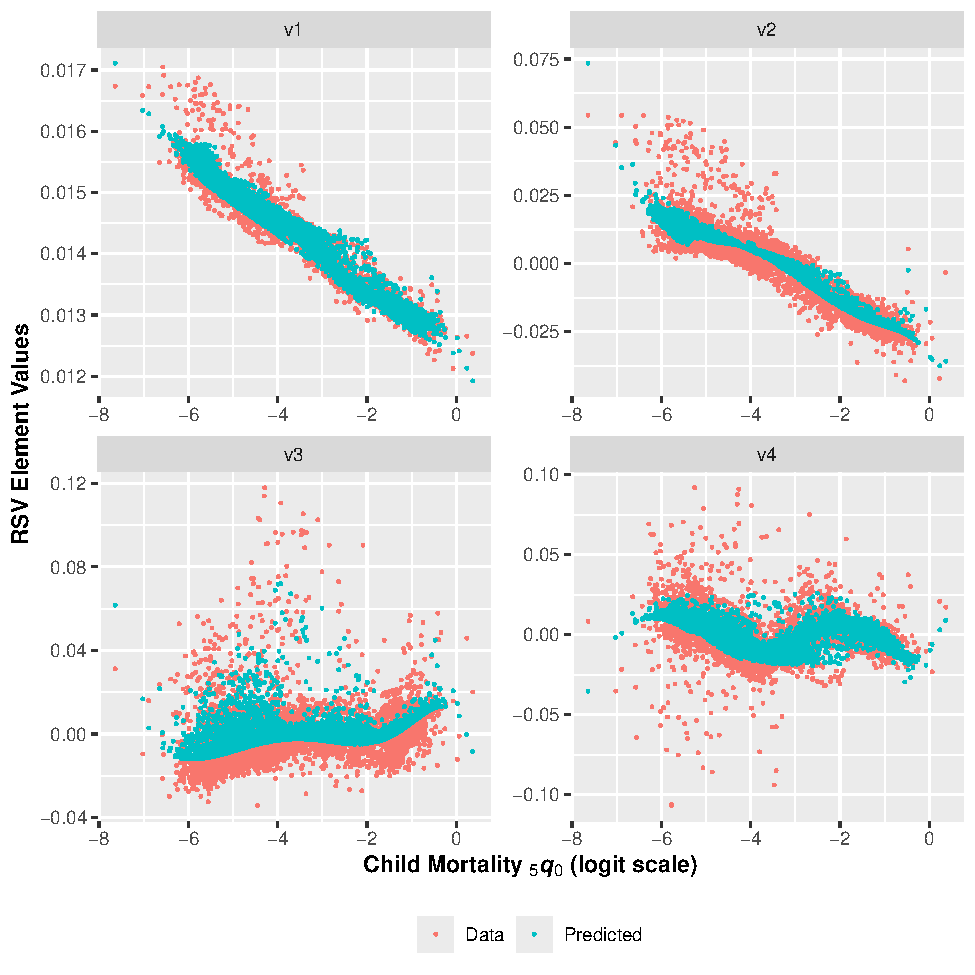
\includegraphics[width=0.94\linewidth]{../figures/fig2-1f.pdf} 
   \captionsetup{format=plain,font=normalsize,margin=0cm,justification=justified}
   \caption{\textbf{Right Singular Vector Element Values for Females.} Values and predictions from model in Equation \ref{eqn:vsByMx} on the logit scale by $\logit(\qf)$.  The predicted values are based on both $\qf$ and $\qff$ which explains why they appear as a cloud rather than a curve.}
   \label{fig:rsvF}
\end{figure}

% Figure male RSV values
\begin{figure}[htbp]
   \centering
   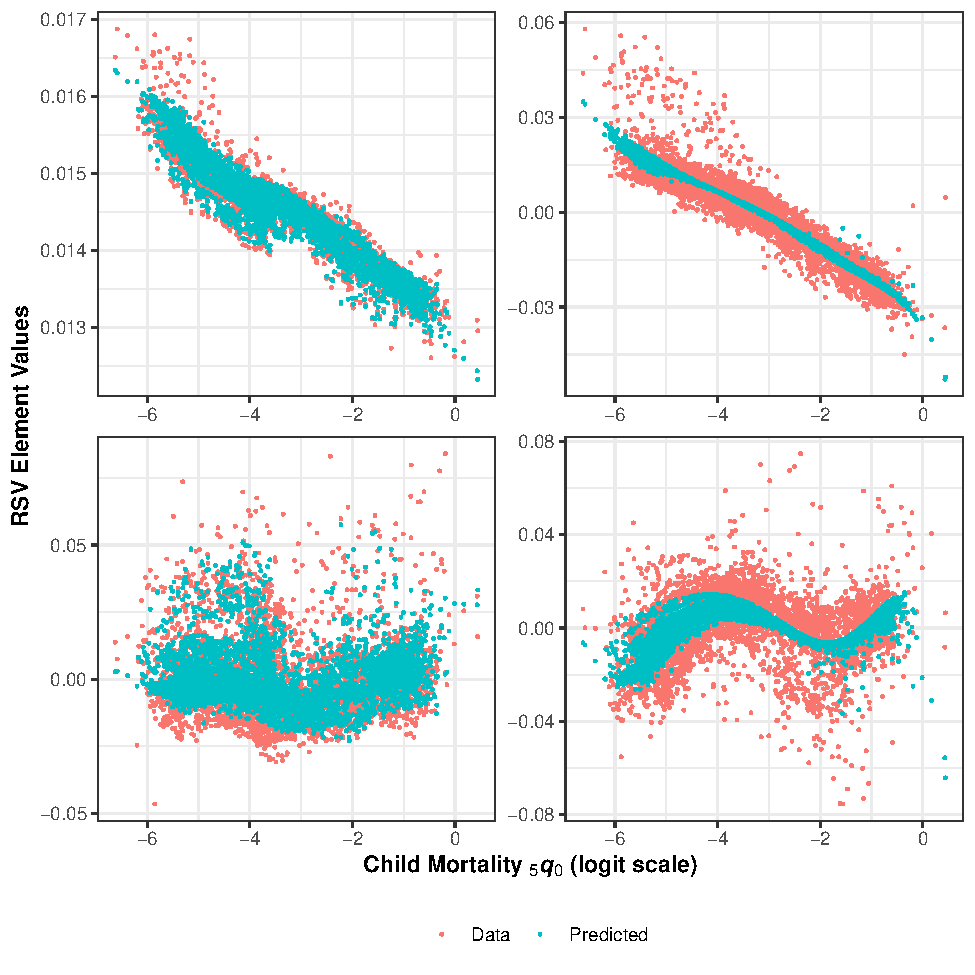
\includegraphics[width=0.94\linewidth]{../figures/fig2-1m.pdf} 
   \captionsetup{format=plain,font=normalsize,margin=0cm,justification=justified}
   \caption{\textbf{Right Singular Vector Element Values for Males.} Values and predictions from model in Equation \ref{eqn:vsByMx} on the logit scale by $\logit(\qf)$.  The predicted values are based on both $\qf$ and $\qff$ which explains why they appear as a cloud rather than a curve.}
   \label{fig:rsvM}
\end{figure}

% Figure adult vs. child mortality
\begin{figure}[htbp]
   \centering
   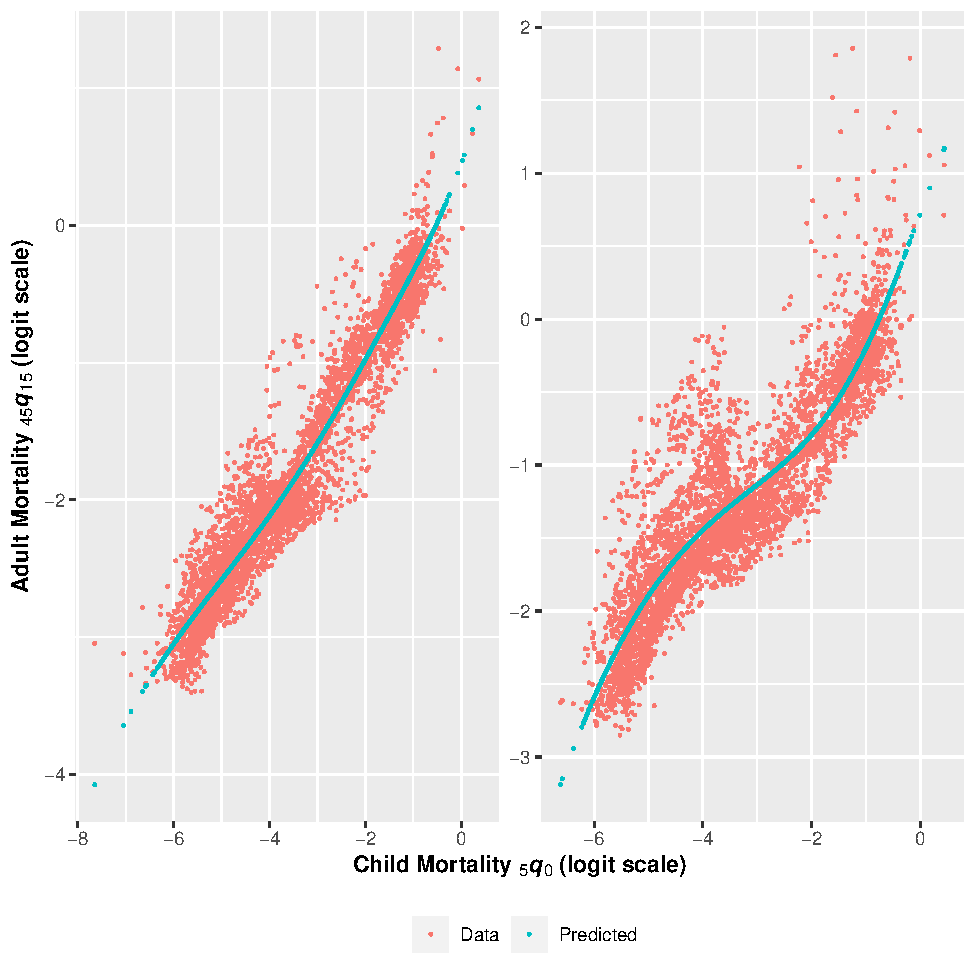
\includegraphics[width=0.94\linewidth]{../figures/fig2-2.pdf} 
   \captionsetup{format=plain,font=normalsize,margin=0cm,justification=justified}
   \caption{\textbf{Adult vs. Child Mortality.} Values and predictions from model in Equation \ref{eqn:amCm} on the logit scale by $\logit(\qf)$.}
   \label{fig:adultChild}
\end{figure}

% Figure first year of life mortality by child mortality
\begin{figure}[htbp]
   \centering
   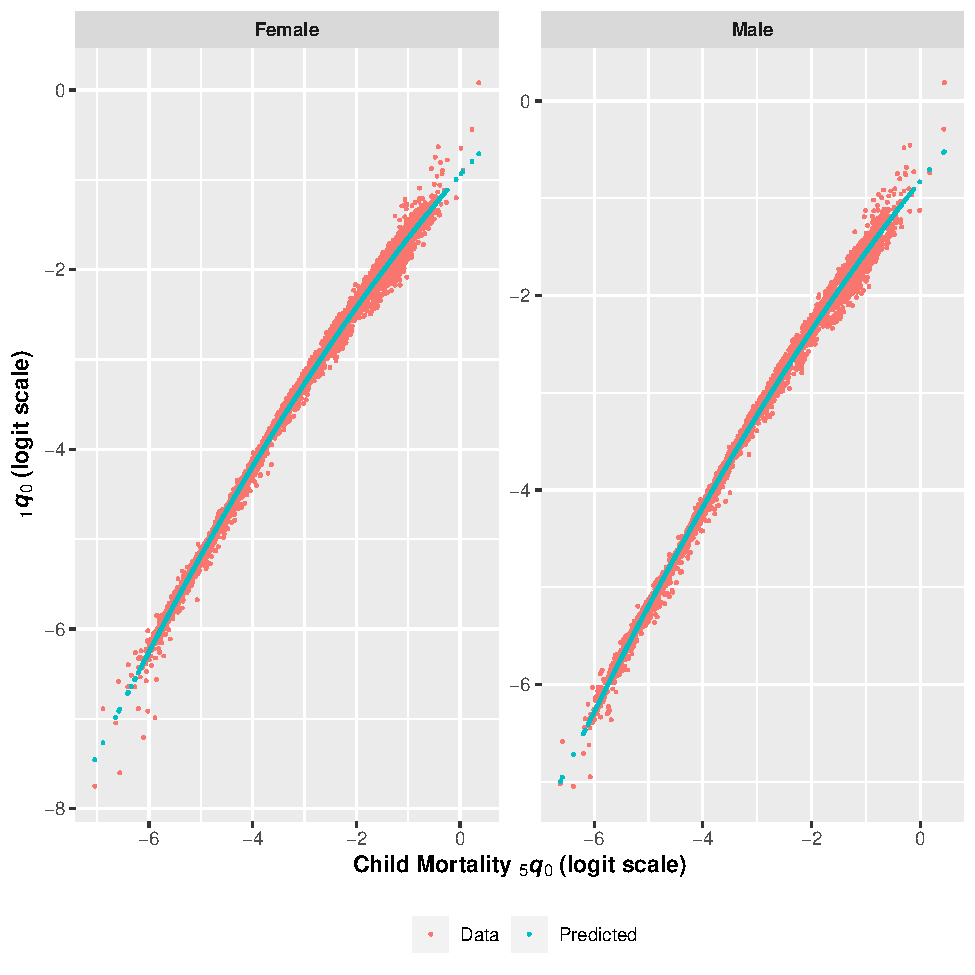
\includegraphics[width=0.94\linewidth]{../figures/fig2-3.pdf} 
   \captionsetup{format=plain,font=normalsize,margin=0cm,justification=justified}
   \caption{\textbf{Age 0 Probability of Dying $\qoz$ vs. Child Mortality.} Values and predictions from model in Equation \ref{eqn:q0Cm} on the logit scale by $\logit(\qf)$.}
   \label{fig:q0Child}
\end{figure}

% Figure example predicted values at various levels of mortality
\begin{figure}[htbp]
   \centering
   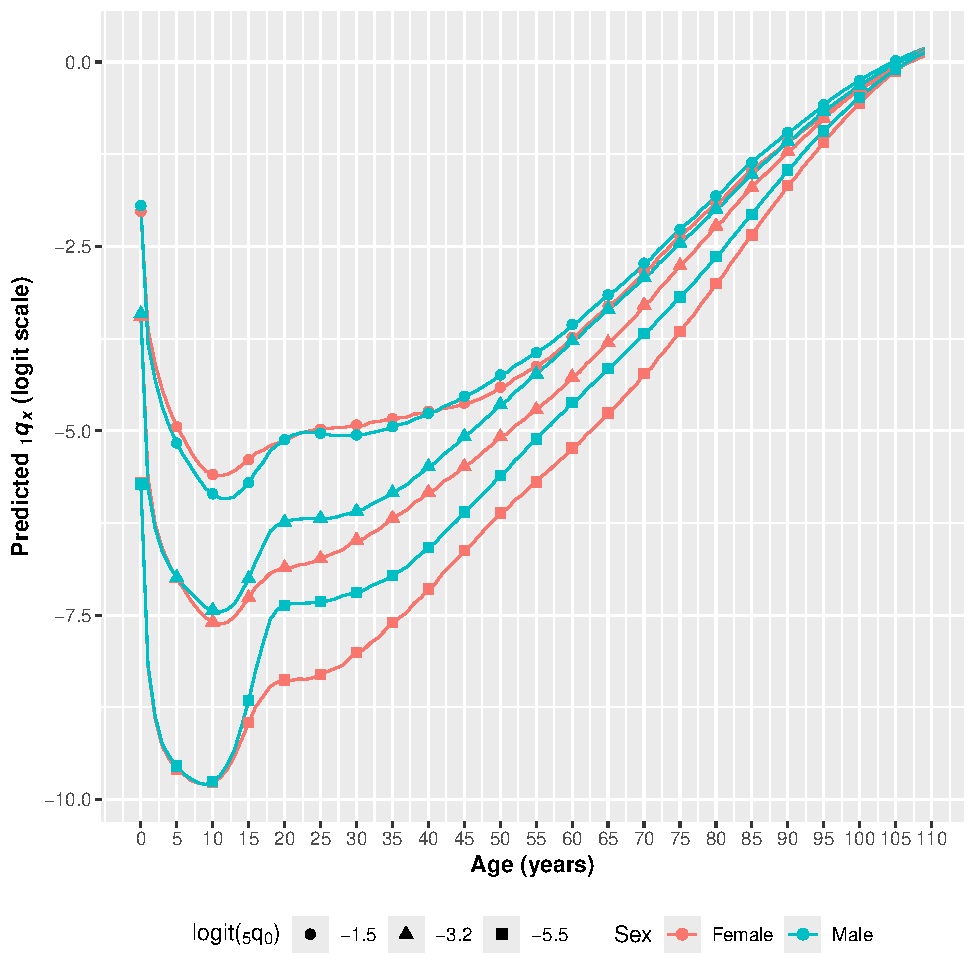
\includegraphics[width=0.94\linewidth]{../figures/fig6.pdf} 
   \captionsetup{format=plain,font=normalsize,margin=0cm,justification=justified}
   \caption{\textbf{Predicted $\qox$ at Three Levels of $\qf$.}  As $\qf$ increases the relationship between female and male mortality changes, and female mortality generally exceeds male mortality between ages roughly 10 and 40 for high levels of $\qf$.  It has been verified that this reflects the real change in this relationship embodied in the HMD life tables.}
   \label{fig:preds}
\end{figure}

% Figure interquartile range of prediction errors
\begin{figure}[htbp]
   \centering
   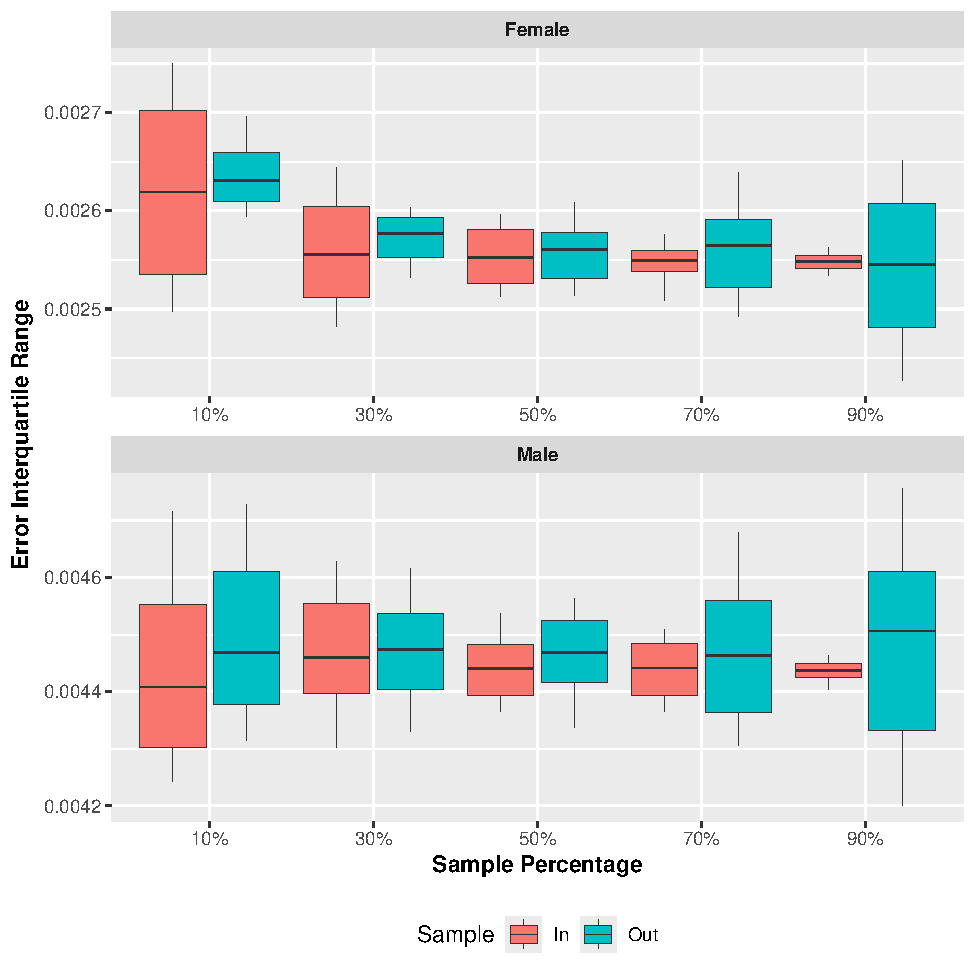
\includegraphics[width=\linewidth]{../figures/fig5b.pdf} 
   \captionsetup{format=plain,font=normalsize,margin=0cm,justification=justified}
   \caption{\textbf{Interquartile Range of Prediction Error by Sample Fraction.}  50 samples for each sample fraction.  For each sample, the interquartile range is calculated across all ages and all mortality schedules in each sample category (in/out).  Whiskers extend to 10\% and 90\% quantiles.}
   \label{fig:iqrSampErr}
\end{figure}


%%% === %%% === %%%
\newpage
\section{Additional Error Summary Tables} \label{app:errorTabs}

\begin{table}[htp]
\captionsetup{format=plain,font=normalsize,margin=1.9cm,justification=justified}
\caption{\textbf{Weighted age-specific absolute errors in $\qfxhat$.} Errors summed across all 4,610 HMD life tables `SC' is SVD-Comp and `LQ' is Log-Quad'.}
\begin{center}
\begin{tabular}{crrrrrr}
  \toprule
  & \multicolumn{3}{c}{Female} & \multicolumn{3}{c}{Male} \\
  \cmidrule(lr){2-4} \cmidrule(lr){5-7}
  $x$ (years) & \multicolumn{1}{c}{SC} & \multicolumn{1}{c}{LQ} & \multicolumn{1}{c}{SC-LQ} & \multicolumn{1}{c}{SC} & \multicolumn{1}{c}{LQ} & \multicolumn{1}{c}{SC-LQ} \\
  \midrule
  \input ../tables/ageCompQ-1.txt
  \midrule
  \input ../tables/ageCompQ-2.txt
   \bottomrule
\end{tabular}
\end{center}
\label{tab:qErrs}
\end{table}%

\begin{table}[htp]
\captionsetup{format=plain,font=normalsize,margin=2cm,justification=justified}
\caption{\textbf{Weighted age-specific absolute errors in $\exhat$.} Errors summed across all 4,610 HMD life tables. `SC' is SVD-Comp and `LQ' is Log-Quad'.}
\begin{center}
\begin{tabular}{crrrrrr}
  \toprule
  & \multicolumn{3}{c}{Female} & \multicolumn{3}{c}{Male} \\
  \cmidrule(lr){2-4} \cmidrule(lr){5-7}
  $x$ (years) & \multicolumn{1}{c}{SC} & \multicolumn{1}{c}{LQ} & \multicolumn{1}{c}{SC-LQ} & \multicolumn{1}{c}{SC} & \multicolumn{1}{c}{LQ} & \multicolumn{1}{c}{SC-LQ} \\
  \midrule
  \input ../tables/ageCompE-1.txt
  \midrule
  \input ../tables/ageCompE-2.txt
   \bottomrule
\end{tabular}
\end{center}
\label{tab:eErrs}
\end{table}%

\begin{table}[htp]
\captionsetup{format=plain,font=normalsize,margin=4cm,justification=justified}
\caption{\textbf{Total Absolute Errors in $\ez$.}}
\begin{center}
\begin{tabular}{lrr}
  \toprule
  Value & Female & Male \\
  \midrule
  \input ../tables/ageCompLQ.txt
  \input../tables/ageCompSVD-Comp.txt
  \input ../tables/ageCompSVD-CompLogQuadDiffs.txt
  \bottomrule
\end{tabular}
\end{center}
\label{tab:e0Errs}
\end{table}%

\end{appendices}

\end{document}  